\renewcommand{\theequation}{\theenumi}
\begin{enumerate}[label=\arabic*.,ref=\thesubsection.\theenumi]
\numberwithin{equation}{enumi}
\item Tangents are drawn to the hyperbola 
\begin{equation}
\vec{x}^TV\vec{x} =36 
\label{eq:hyper}
\end{equation}
%
where
\begin{equation}
V = \myvec{4 & 0 \\ 0 & -1}
\label{eq:hyperv}
\end{equation}
%
at points $\vec{P}$ and $\vec{Q}$.  If these tangents intersect at 
\begin{equation}
\vec{T}= \myvec{0 \\ 3},
\end{equation}
%
find the equation of $PQ$.
\\
\solution The equations of the two tangents are obtained using \eqref{eq:tangent} as
\begin{align}
\vec{P}^TV\vec{x} &=36
\\
\vec{Q}^TV\vec{x}  &=36.
\end{align}		
%
Since both pass through $\vec{T}$
\begin{align}
\label{eq:hyperp}
\vec{P}^TV\vec{T}  &=36 \implies \vec{P}^T\myvec{0  \\  -3} = 36
\\
\vec{Q}^TV\vec{T}  &=36 \implies \vec{Q}^T\myvec{0  \\  -3} = 36
\label{eq:hyperq}
\end{align}
Thus, $\vec{P}, \vec{Q}$ satisfy
\begin{align}
\myvec{0 &  -3}\vec{x} &= -36
\\
\implies \myvec{0 &  1}\vec{x} &= -12
\label{eq:d1}
\end{align}
%
which is the equation of $PQ$.
\item In $\triangle PTQ$, find the equation of the altitude $TD \perp PQ$.
\\
\solution Since 
\begin{align}
 \myvec{1 &  0} \myvec{0 \\  1}=0
\end{align}
using \eqref{eq:line_normal} and \eqref{eq:d1},
the equation of $TD$ is
\begin{align}
\myvec{1 & 0}\brak{\vec{x}-\vec{T}} &= 0
\\
\implies \myvec{1 & 0}\vec{x} &= 0
\label{eq:d2}
\end{align}
%
\item Find $D$.
\\
\solution
From \eqref{eq:d1} and \eqref{eq:d2},
\begin{align}
 \myvec{1 & 0 \\ 0 &  1}\vec{D} &= \myvec{0 \\ -12 }
\\
\implies  \vec{D} &= \myvec{0 \\ -12 }
\label{eq:hyperd}
\end{align}
%
\item Show that the equation of $PQ$ can also be expressed as
\begin{align}
\label{eq:pq_slope}
\vec{x} = \vec{D}+\lambda \vec{m}
\end{align}
where
\begin{align}
\vec{m} &=   \myvec{1 \\ 0}
\label{eq:hyper_slope}
\end{align}
%
\item Show that for $\vec{V}^T = \vec{V}$,
\begin{equation}
\label{eq:quad_md}
\brak{\vec{D}+\lambda\vec{m}}^TV\brak{\vec{D}+\lambda\vec{m}} + F= 0 
\end{equation}
can be expressed as
\begin{equation}
\label{eq:quad_lambda}
\lambda^2\vec{m}^TV\vec{m}+2\lambda\vec{m}^TV\vec{D}+\vec{D}^TV\vec{D}
+ F = 0
\end{equation}
%
\item Find $\vec{P}$ and $\vec{Q}$.
\\
\solution From \eqref{eq:pq_slope} and \eqref{eq:hyper} \eqref{eq:quad_lambda} is obtained.
%
Substituting from \eqref{eq:hyper_slope}, \eqref{eq:hyperv} and \eqref{eq:hyperd}
\begin{align}
\vec{m}^TV\vec{m} &= \myvec{1& 0} \myvec{4 & 0 \\ 0 & -1}\myvec{1 \\ 0} = 4
\\
\vec{m}^TV\vec{D} & = \myvec{1& 0}\myvec{4 & 0 \\ 0 & -1}\myvec{0 \\ -12 } = 0
\\
\vec{D}^TV\vec{D} &= \myvec{0 & -12 }\myvec{4 & 0 \\ 0 & -1}\myvec{0 \\ -12 } = -144
\end{align}
%
Substituting in \eqref{eq:quad_lambda}
\begin{align}
4 \lambda^2 - 144 &= 36
\\
\implies
\lambda &= \pm 3\sqrt{5}
\end{align}
%
Substituting in \eqref{eq:pq_slope},
\begin{align}
\vec{P} &= \vec{D}+ 3\sqrt{5} \vec{m} = 3 \myvec{ \sqrt{5} \\ -4}
\\
\vec{Q} &= \vec{D}- 3\sqrt{5} \vec{m} = -3 \myvec{ \sqrt{5} \\ 4}
\end{align}
%
\item Find the area of $\triangle PTQ$.
\\
\solution Since
\begin{align}
PQ &= \norm{\vec{P}-\vec{Q}} = 6\sqrt{5}
\\
TD &= \norm{\vec{T}-\vec{D}} = 15,
\end{align}
the desired area is
\begin{equation}
\frac{1}{2}PQ \times TD = 45 \sqrt{5}
\end{equation}
\item Repeat the previous exercise using determinants.
\item 
%Summarize all the above computations through a Python script and 
Plot 
the hyperbola.
\\
\solution  See Fig. \ref{fig:hyperbola}
\begin{figure}
\centering
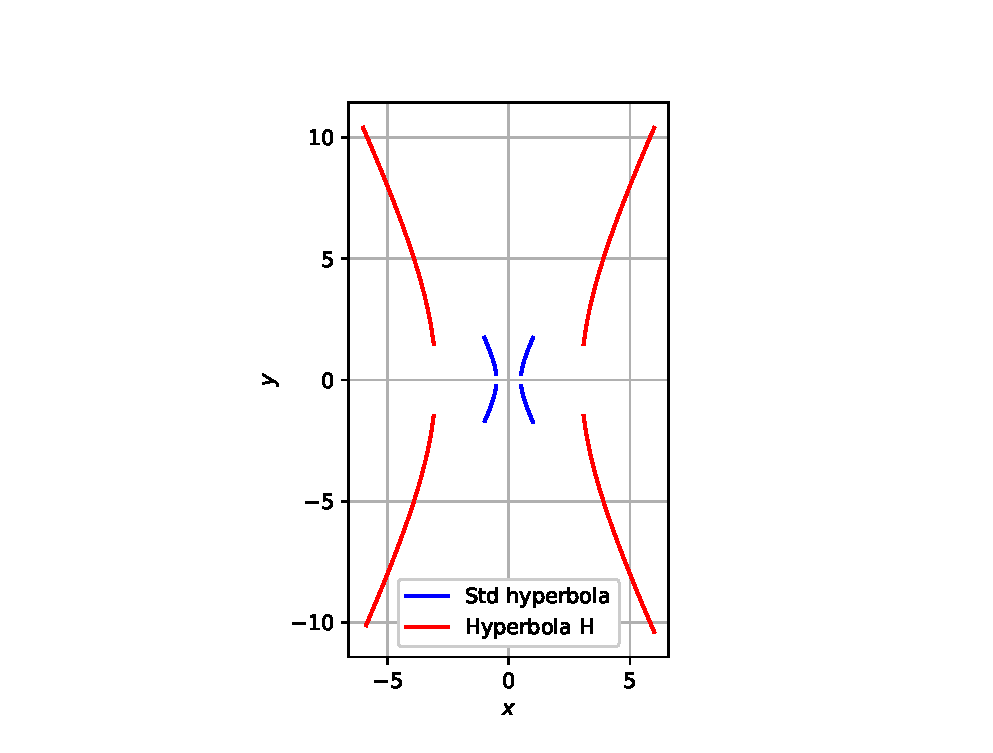
\includegraphics[width=\columnwidth]{./figs/hyperbola.eps}
\caption{}
\label{fig:hyperbola}
\end{figure}

\end{enumerate}

